\chapter{\IfLanguageName{dutch}{Stand van zaken}{State of the art}}%
\label{ch:stand-van-zaken}

% Tip: Begin elk hoofdstuk met een paragraaf inleiding die beschrijft hoe
% dit hoofdstuk past binnen het geheel van de bachelorproef. Geef in het
% bijzonder aan wat de link is met het vorige en volgende hoofdstuk.

% Pas na deze inleidende paragraaf komt de eerste sectiehoofding.

Dit hoofdstuk bevat je literatuurstudie. De inhoud gaat verder op de inleiding, maar zal het onderwerp van de bachelorproef *diepgaand* uitspitten. De bedoeling is dat de lezer na lezing van dit hoofdstuk helemaal op de hoogte is van de huidige stand van zaken (state-of-the-art) in het onderzoeksdomein. Iemand die niet vertrouwd is met het onderwerp, weet nu voldoende om de rest van het verhaal te kunnen volgen, zonder dat die er nog andere informatie moet over opzoeken \autocite{Pollefliet2011}.

Je verwijst bij elke bewering die je doet, vakterm die je introduceert, enz.\ naar je bronnen. In \LaTeX{} kan dat met het commando \texttt{$\backslash${textcite\{\}}} of \texttt{$\backslash${autocite\{\}}}. Als argument van het commando geef je de ``sleutel'' van een ``record'' in een bibliografische databank in het Bib\LaTeX{}-formaat (een tekstbestand). Als je expliciet naar de auteur verwijst in de zin (narratieve referentie), gebruik je \texttt{$\backslash${}textcite\{\}}. Soms is de auteursnaam niet expliciet een onderdeel van de zin, dan gebruik je \texttt{$\backslash${}autocite\{\}} (referentie tussen haakjes). Dit gebruik je bv.~bij een citaat, of om in het bijschrift van een overgenomen afbeelding, broncode, tabel, enz. te verwijzen naar de bron. In de volgende paragraaf een voorbeeld van elk.

\textcite{Knuth1998} schreef een van de standaardwerken over sorteer- en zoekalgoritmen. Experten zijn het erover eens dat cloud computing een interessante opportuniteit vormen, zowel voor gebruikers als voor dienstverleners
 op vlak van informatietechnologie~\autocite{Creeger2009}.

Let er ook op: het \texttt{cite}-commando voor de punt, dus binnen de zin. Je verwijst meteen naar een bron in de eerste zin die erop gebaseerd is, dus niet pas op het einde van een paragraaf.


\begin{figure}
  \centering
  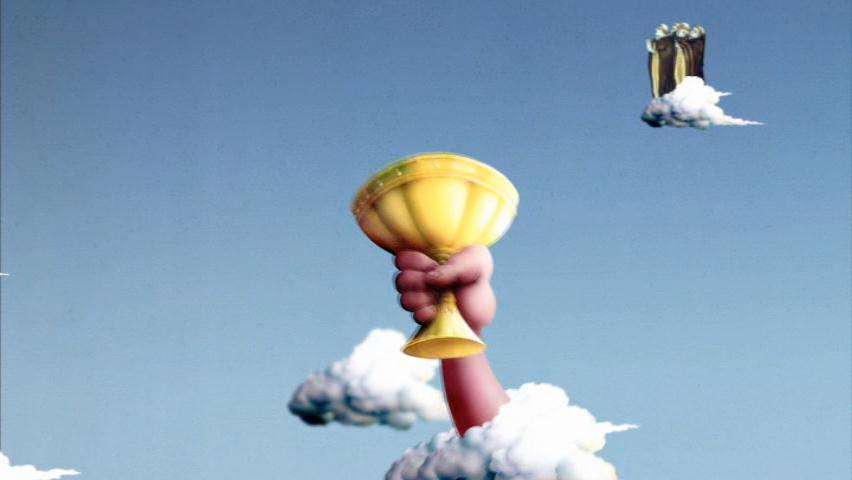
\includegraphics[width=0.8\textwidth]{grail.jpg}
  \caption[Voorbeeld figuur.]{\label{fig:grail}Voorbeeld van invoegen van een figuur. Zorg altijd voor een uitgebreid bijschrift dat de figuur volledig beschrijft zonder in de tekst te moeten gaan zoeken. Vergeet ook je bronvermelding niet!}
\end{figure}

\begin{listing}
  \begin{minted}{python}
    import pandas as pd
    import seaborn as sns

    penguins = sns.load_dataset('penguins')
    sns.relplot(data=penguins, x="flipper_length_mm", y="bill_length_mm", hue="species")
  \end{minted}
  \caption[Voorbeeld codefragment]{Voorbeeld van het invoegen van een codefragment.}
\end{listing}


\begin{table}
  \centering
  \begin{tabular}{lcr}
    \toprule
    \textbf{Kolom 1} & \textbf{Kolom 2} & \textbf{Kolom 3} \\
    $\alpha$         & $\beta$          & $\gamma$         \\
    \midrule
    A                & 10.230           & a                \\
    B                & 45.678           & b                \\
    C                & 99.987           & c                \\
    \bottomrule
  \end{tabular}
  \caption[Voorbeeld tabel]{\label{tab:example}Voorbeeld van een tabel.}
\end{table}




Het 13F formulier van de Securities and Exchange Commission (SEC) is een rapport dat institutionele vermogensbeheerders elk kwartaal moeten indienen als ze voor meer dan \$100 miljoen of meer aan Section 13(f) effecten bezitten. Sectie 13(f) van de Securities Exchange Act van 1934 legt deze verplichting op met als doel de transparantie van het effectenbezit van grote institutionele beleggers te vergroten. In 1975 implementeerde het Congres deze bepaling om de toegankelijkheid van informatie over de investeringsactiviteiten van deze bedrijven te verbeteren. Ze geloofden dat dit openbaarmakingsprogramma het vertrouwen van beleggers in de integriteit van de effectenmarkten van de Verenigde Staten zou versterken~\autocite(SECform13F2024).\\
Formulier 13F biedt een uitgebreid overzicht van de aandelenbeleggingen van prominente beleggingsentiteiten wereldwijd, waardoor het een uiterst belangrijk hulpmiddel is voor analisten, onderzoekers en beleggers die inzicht willen krijgen in markttrends en de beleggingsbenaderingen van belangrijke marktspelers. Het onverwerkte tekstuele formaat waarin deze inzendingen worden aangeleverd, vormt echter een aanzienlijke belemmering voor effectieve gegevensextractie en -analyse.\\
Kunstmatige intelligentie (AI) en Machine Learning (ML) technologieën hebben de extractie en organisatie van gegevens uit ongestructureerde tekst de afgelopen jaren aanzienlijk veranderd. Geavanceerde methodologieën zoals Natural Language Processing (NLP) en deep learning modellen maken het mogelijk om tekstuele 13F aanvragen om te zetten in gestructureerde datasets die geschikt zijn voor grondige analyse en studie. Vervolgens kunnen deze georganiseerde gegevens worden opgeslagen in databases, zodat ze eenvoudiger kunnen worden opgevraagd, weergegeven en onderzocht.\\
\\
Het doel van deze literatuurstudie is het onderzoeken en beoordelen van de verschillende Artificial Intelligence (AI) en Machine Learning (ML) technieken die kunnen worden gebruikt om gegevens uit 13F-formulieren te extraheren, te organiseren en op te slaan. Het doel van het onderzoek is het bepalen van de meest efficiënte methoden om de ongeorganiseerde inhoud van deze documenten om te zetten in een gestructureerd formaat dat geschikt is voor analyse en opslag in een database. Dit houdt in dat er een vergelijkend onderzoek wordt gedaan naar verschillende kunstmatige intelligentie methodologieën, zoals Natural Language Processing (NLP) en Deep Learning modellen, en dat bepaalde tools zoals BERT, GPT en SpaCy worden geëvalueerd. De evaluatie zal ook de integratie van gestructureerde gegevens in databasemanagementsystemen (DBMS) onderzoeken, om te garanderen dat de geëxtraheerde gegevens gemakkelijk beschikbaar zijn voor later onderzoek en analyse. Het doel van deze evaluatie is om een uitgebreide kennis te krijgen van de meest effectieve procedures en technologie voor het verwerken van 13F-formulieren. 

% ----------------------------------------------------------------------------
\section{Wat zijn 13F meldingen}
\subsection{Definitie en doel}
\subsection{Structuur en inhoud}
% ----------------------------------------------------------------------------
\section{AI- en Tekstextractietechnieken}
\subsection{Natural Language Processing (NLP)}
\subsection{Machine Learning (ML) benaderingen}
% ----------------------------------------------------------------------------
\subsection{Vergelijkende analuse van techologiën}
To be reviewed
% ----------------------------------------------------------------------------
\section{Technieken en Tools}
\subsection{Tekstverwerkingtools}
\subsection{Database Management Systemen (DBMS)}
\subsection{ETL Tools}
% ----------------------------------------------------------------------------
\section{Uitdagingen en beperkingen}
\subsection{Camplexiteit van financiële Tekst}
\subsection{Gegevenskwaliteit en Validatie}
\subsection{Databaseprestaties}
% ----------------------------------------------------------------------------
\section{Leemtes in huidig onderzoek}
\subsection{Onbehandelde kwesties}
\subsection{Verbeteringsmogelijkehden}

% ----------------------------------------------------------------------------
\section{Toekomstige richtingen}
\subsection{Voortgang in AI en NLP}
\subsection{Integration with financiele analyse}
% ----------------------------------------------------------------------------
\section{conclusie}
\subsection{Samenvatting van Bevindingen}
\subsection{Implicaties van het onderzoek}